\chapter{Предлагаемый метод}
\label{chapter_method}

В ходе работы был разработан и реализован программный модуль, реализующий поискового робота. В разделе \ref{strategy} описана предлагаемая стратегия приоритезации, а в разделе \ref{steps} описаны основные этапы алгоритма работы поискового робота.

\section{Стратегия приоритезации}
\label{strategy}

Основная идея стретегии приоритезации заключается в объединении стратегии отбора и стратегии повторного обхода посредством введения единого значения $VRank$ (visit rank). Вычисление такого ранга для веб-страницы $p$ осуществляется по следующей формуле:
$$VRank(p) = QRank(p) * RVRank(p)$$
где $QRank(p)$ --- эвристическая важность страницы, то есть ранг, характеризующий ее качество (quality rank), а $RVRank(p)$ --- ранг, характеризующий необходимость повторно скачивать веб-страницу $p$ (re-visit rank). 

Как было сказано в разделе \ref{selection_strategy}, стратегии отбора, располагающие информацией о рангах веб-страниц, находят важные страницы раньше, чем стратегии, использующие информацию, полученную только в процессе текущего обхода. Потому для вычисления $QRank$ предлагается использовать <<оракула>>, который сообщал бы ранги веб-страниц, найденных во время обхода. Поскольку информацией о полном веб-графе мы не располагаем, будет использовать метод машинного обучения, который можно отнести к категории поточечных подходов обучения ранжированию, описание которой есть в разделе \ref{learning_to_rank}. Суть метода заключается в использовании нейронной сети, задача которой --- по URL-адресу веб-страницы получить число, имеющее смысл эвристической оценки важности страницы. Для чего на основании URL-адреса строится вектор статических особенностей, список которых представлен в разделе \ref{static_features}. Нейронная сеть принимает на вход этот вектор и вычисляет ранг веб-страницы.

Для вычисления $QRank$ предлагается два метода. Первый базируется исключительно на статических особенностях URL-адреса, и для каждой веб-страницы $QRank$ вычисляется один раз при добавлении адреса в коллекцию. Второй также использует свойства веб-графа, а именно, после обработки скачананной страницы, ее $QRank$ распределяется между страницами, ссылки на которые она содержит. Таким образом, при добавлении нового URL-адреса $QRank$ считается при помощи нейронной сети, а затем он может изменятся в процессе дальнейшей работы.

Метод вычисления $RVRank$ основан на следующей идее. Заново обходить веб-страницы следует с частотой, пропорциональной частоте их изменения, потому для каждой страницы необходимо определить период ее изменения. Это осуществляется посредством итеративного приближения, то есть уточнения значения периода измения страницы при каждом ее скачивании. Кроме того, следует учитывать, что существуют динамические страницы, которые генерируются заново при переходе по URL-адресу. Динамические страницы не следует скачивать бесконечно часто. Это осуществляется, во-первых, за счет вероятного небольшого значения $QRank$ таких страниц, а во-вторых, путем введения нижней границы для значения периода изменения. Таким образом, при повторном скачивании страницы, необходимо проверить, была ли она изменена с момента предыдущего посещения и, если да, уменьшить предполгаемый период изменения (если он не достиг нижней границы), в противном же случае --- увеличить.

\section{Этапы алгоритма}
\label{steps}

Основные компоненты разработанного поискового робота представлены на рисунке \ref{architecture}.

\begin{figure}[h!]
\center{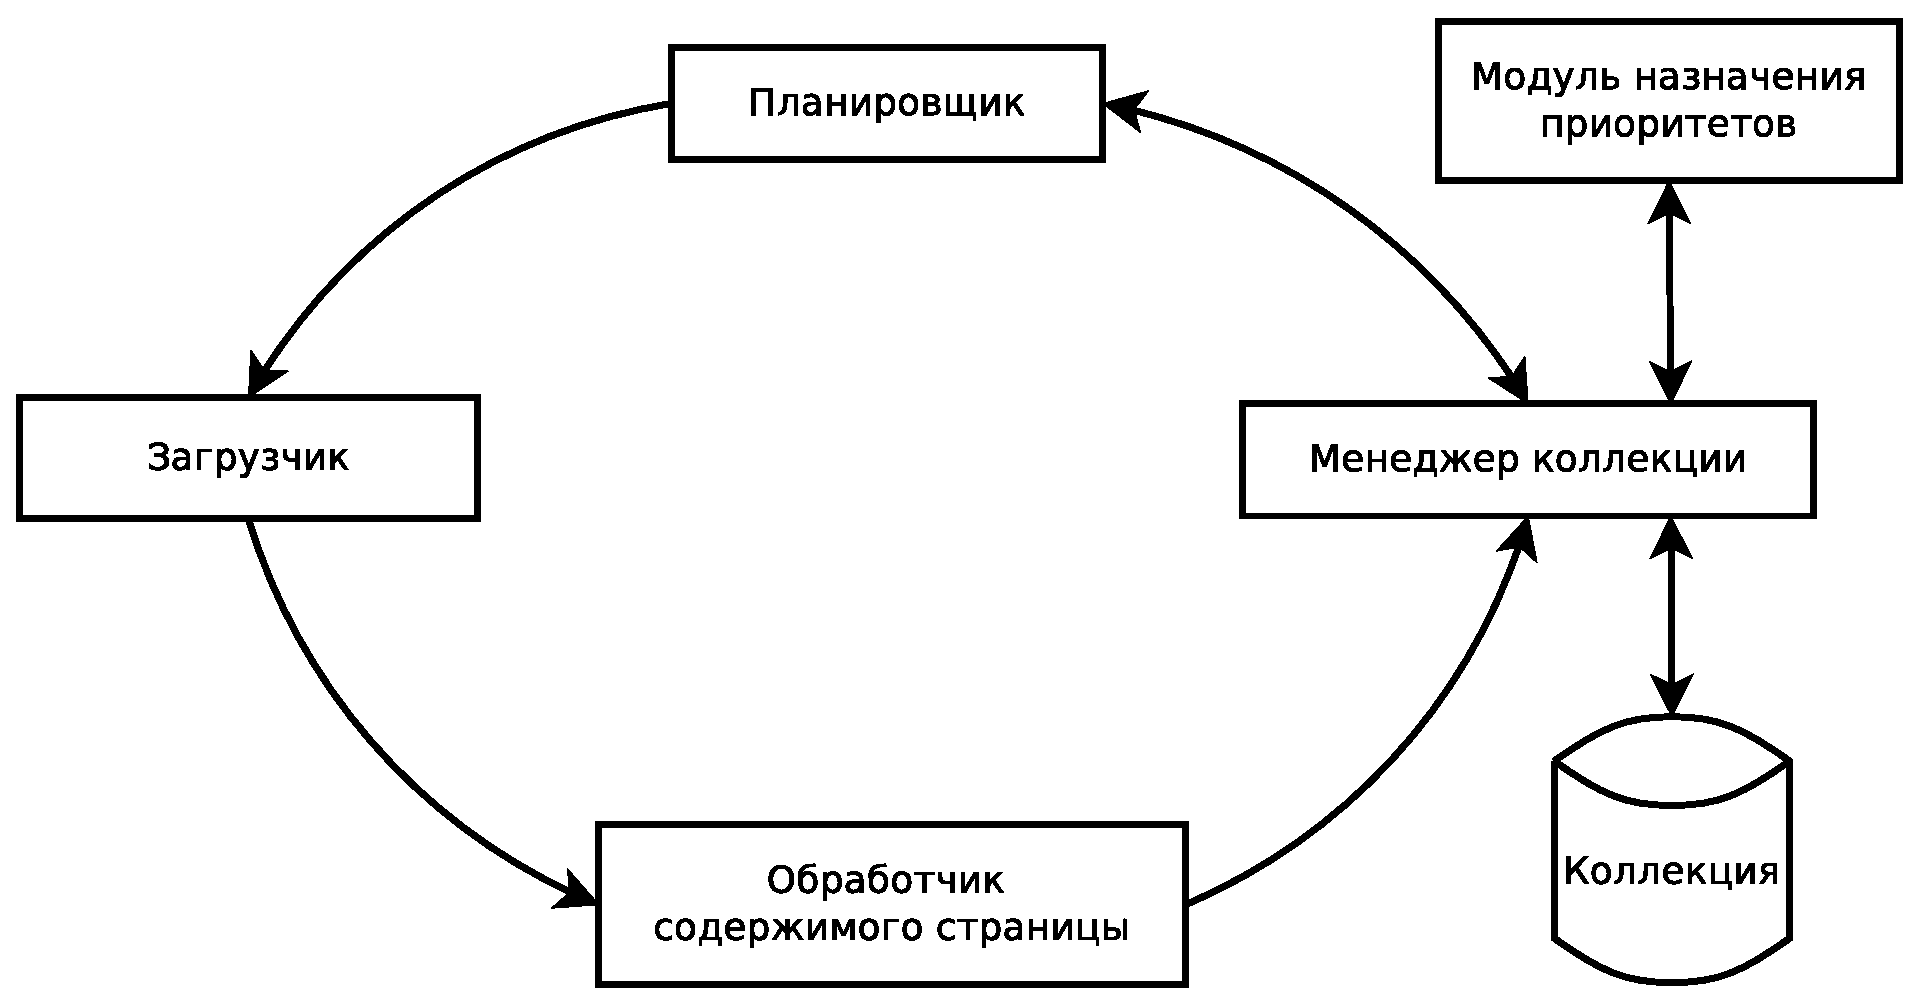
\includegraphics[width=1\linewidth]{pics/architecture.eps}}
\caption{Основные программные компоненты поискового робота}
\label{architecture}
\end{figure}

Алгоритм включает в себя два этапа: подготовительный  и основной. На подготовительном этапе происходит инициализация модуля назначения приоритетов, а на основном --- непосредственно обход интернета. Рассмотрим подробнее каждый из этапов.

\subsection*{Подготовительный этап}

На подготовительном этапе производится обучение нейронной сети, которая входит в модуль назначения приоритетов. В качестве обучающего множества используется набор URL-адресов веб-страниц с известными рангами (например, $PageRank$). Затем в коллекцию добавляется стартовое множество URL-адресов, и для каждого из них вычисляется $QRank$.

\subsection*{Основной этап}

Работа алгоритма на основном этапе происходит циклически. На каждом шаге цикла обрабатывается $K$ страниц из коллекции, имеющих наибольший $VRank$. 

Цикл начинается с того, что планировщик запрашивает у менеджера коллекции следующую партию адресов веб-страниц. После чего происходит подсчет $VRank$ для каждой страницы из коллекции посредством запросов менеджера коллекции к модулю приоритезации. Затем менеджер коллекции формирует партию, содержащую $K$ адресов веб-страниц, имеющих наибольший $VRank$ и отдает ее планировщику. После чего планировщик последовательно передает URL-адреса для дальнейшей обработки. 

Обработка начинается с загрузки веб-страницы, получаемой по текущему URL-адресу. Следует помнить, что при загрузке следует учитывать правила вежливости, описанные в разделе \ref{spider}, и в любой момент времени с каждым хостом должно быть установлено не более одного соединения. После загрузки следует проверить, обновилась ли страница с момента предыдущего посещения, чтобы осуществить пересчет предполагаемого периода обновления для текущей страницы. После чего обработчик содержимого страницы извлекает ссылки с загруженной веб-страницы, нормализует их и передает полученые URL-адреса менеджеру коллекции. После чего модулем приоритезации рассчитываются $QRank$ для каждого URL-адреса, извлеченного с текущей страницы.

Когда все $K$ страниц из текущей партии будут обработаны, алгоритм перейдет к следующему шагу цикла.

\section{Статические особенности URL-адреса}
\label{static_features}

Для вычисления $QRank$ веб-страницы были использованы следующие статические особенности ее URL-адреса. Они были разделены на четыре группы.

\subsection*{Особенности длины}

В эту группу включены особенности, характеризующие длины компонент URL-адреса. Такие как:

\begin{itemize}
\item Суммарное число символов URL-адреса;
\item Число символов схемы URL-адреса;
\item Число символов хоста;
\item Число символов пути;
\item Число символов запроса.
\end{itemize}

\subsection*{Орфографические особенности}

В эту группу включены особенности, характеризующие орфографические свойства URL-адреса и его компонент. Такие как:

\begin{itemize}
\item Суммарное число цифр, входящих в URL-адрес;
\item Суммарное число заглавных букв, входящих в URL-адрес;
\item Число цифр, содержащихся в хосте;
\item Число цифр, содержащихся в пути URL-адреса;
\item Число цифр, содержащихся в запросе URL-адреса;
\item Число заглавных букв, содержащихся в пути URL-адреса;
\item Число заглавных букв, содержащихся в запросе URL-адреса.
\end{itemize}

\subsection*{Количественные особенности термов}

В данную группу включены особенности, характезующие количество термов в URL-адресе и его компонентах. Разделение на термы осуществлялось посредством разбиения адреса по символом, не являющимися буквами или цифрами. После чего выделялись следующие особенности:

\begin{itemize}
\item Суммарное число термов URL-адреса;
\item Число термов хоста;
\item Число термов пути;
\item Число термов запроса.
\end{itemize}

\subsection*{Словарные особенности термов}

В эту группу включены компоненты, характеризующие частоту реальных слов в компонентах URL-адреса. А именно:

\begin{itemize}
\item Частота реальных слов среди термов, входящих в путь URL-адреса;
\item Частота реальных слов среди термов, входящих в запрос.
\end{itemize}
